%
% file: localoperator.tex
% author: Victor Brena
% description: Briefly describes properties of the local operator.
%

\chapter{Appendix A}
\label{app:app01}

\begin{table}[h]
\centering
\begin{tabular}{ l | c | c | c | c | c }
	\hline
	\textbf{Variable} & \textbf{Num. of Obs.} & \textbf{Mean} & \textbf{Std. Dev.} & \textbf{Minimum} & \textbf{Maximum} \\
    \hline \hline
    Gross Profits & 384,141 & 410.56 & 2,545.95 & -76,735 & 128,130 \\
	\hline
    Total Assets & 402,877 & 4,128.37 & 50,536 & 0 & 3,771,200 \\
    \hline
    Capital Expenditures & 361,750 & 110.67 & 801.49 & -994 & 65,028 \\
    \hline
    R\&D Expense & 164,746 & 54.77 & 382.86 & -0.546 & 14,035.29 \\
    \hline \hline
\end{tabular}
\mycaption[Summary Statistics of Gross Profits, Capital Expenditures, R\&D Expenses, and Total Assets.]{Summary Statistics of Gross Profits, Capital Expenditures, R\&D Expenses, and Total Assets, in Millions of US Dollars.}
\end{table}

\begin{figure}[h]
\begin{minipage}{3.3cm}
    \centering
    \subtop[]{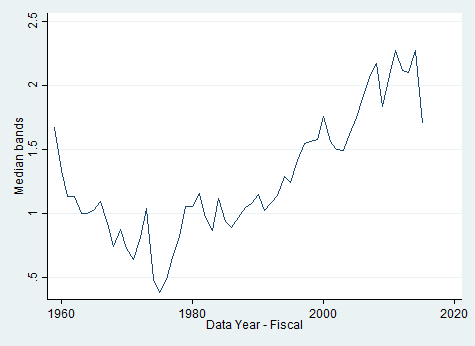
\includegraphics[height=0.3\textheight]{figApp/lcapx_median_graph}\label{Time series plot of median logged capital expenditures.}}
\end{minipage}
\hspace{5cm}
\begin{minipage}{3.3cm}
    \centering
    \subtop[]{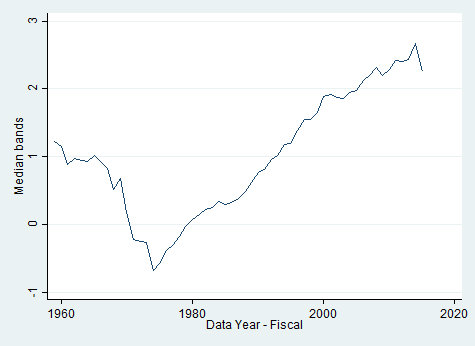
\includegraphics[height=0.3\textheight]{figApp/lxrd_median_graph}\label{Time series plot of median logged R and D expenses.}}
\end{minipage}

\begin{minipage}{3.3cm}
    \centering
    \subtop[]{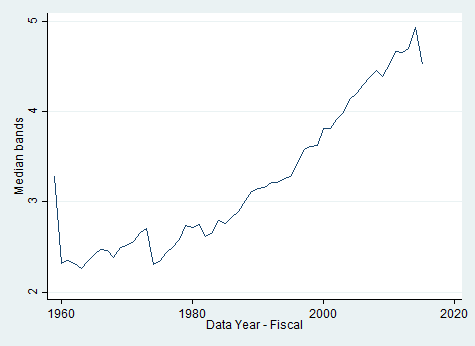
\includegraphics[height=0.3\textheight]{figApp/lgp_median_graph}\label{Time series plot of median logged gross profits.}}
\end{minipage}
\hspace{5cm}
\begin{minipage}{3.3cm}
    \centering
    \subtop[]{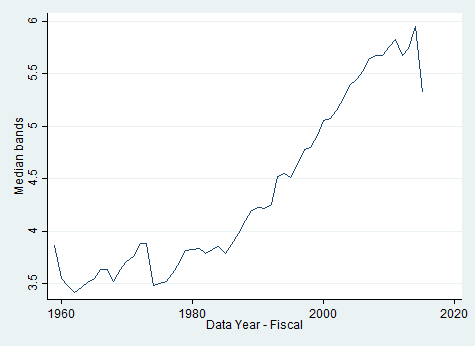
\includegraphics[height=0.3\textheight]{figApp/lat_median_graph}\label{Time series plot of median logged total assets.}}
\end{minipage}

\mycaption[Time Series Plots in Investment, Assets, and Profit Variables.]{(a)~Time series plot of median logged capital expenditures. (b)~Time series plot of median logged research and development expenses. (c)~Time series plot of median logged gross profits. (d)~Time series plot of median logged total assets. }
\label{fig:multiRH02}
\end{figure}

\iffalse
\begin{table}[h]
\begin{tabular}{ c | c }
	\hline
	\textbf{Model 2} \\
    \textbf{Non-Manufacturing Industries} \\
    \textbf{Regressand: Gross Profits} \\
    \hline \hline
    Number of Observations & 698 \\
	\hline
    $R^{2}$ & 0.981 \\
    Adjusted $R^{2}$ & 0.980 \\
    \hline
    $F(45, 652)$ & 745.84 \\
    $Prob > F$ & 0.0000 \\
    \hline \hline
\end{tabular} \\

\begin{tabular}{ l | c | c | c | c | c }
	\hline
	\textbf{Regressors} & \textbf{Estimators} & \textbf{Std. Errors} & $t$ & $P > |t|$ & 95\% CI \\
    & $\hat{\beta}$ & $\hat{\sigma}$ & & & \\
    \hline \hline
	Total Assets & 0.0401 & 0.000225 & 177.85 & 0.000 & (0.0396, 0.0405) \\
	\hline
    Per Cent of Revenue Held & 8.327 & 1.533 & 5.43 & 0.000 & (5.317, 11.338) \\
    By Industry’s Top 50 Firms & & & & & \\
    \hline
    \hline \hline
\end{tabular}
\mycaption[OLS Estimation of Model (2): Coefficients for Main Regressors, Controlling for Year and Industry Fixed Effects (Not Shown)]{OLS Estimation of Model (2): Coefficients for Main Regressors, Controlling for Year and Industry Fixed Effects (Not Shown)}
\end{table}
\fi

\clearpage
\begin{figure}[h]
\begin{minipage}{3.3cm}
    \centering
    \subtop[]{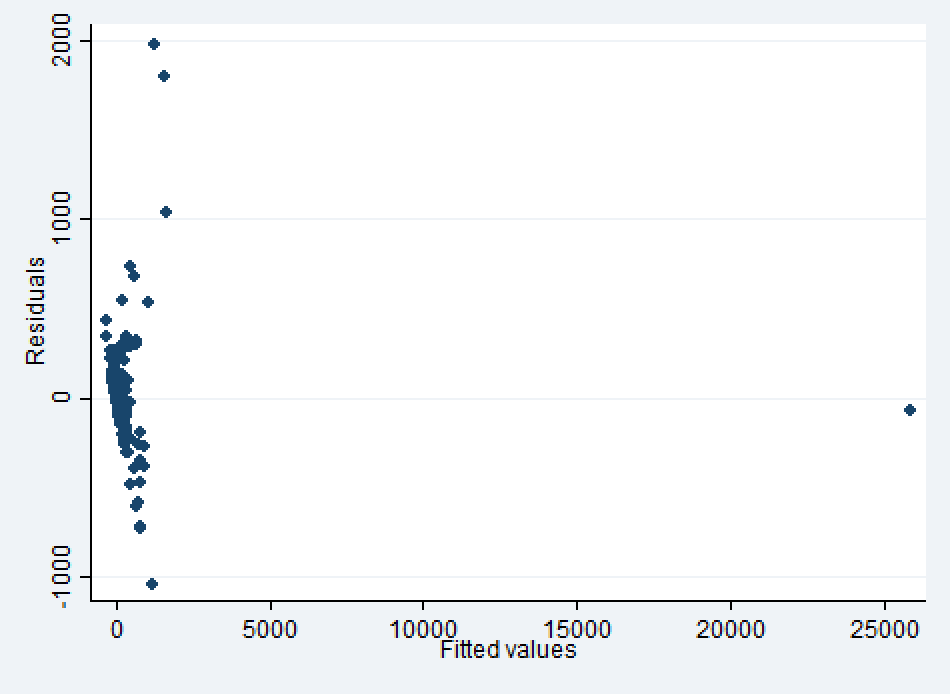
\includegraphics[height=0.3\textheight]{figApp/Model-2-2002-resid}\label{Residuals Plot of OLS Estimation of Model (2) (for Year 2002).}}
\end{minipage}
\hspace{5cm}
\begin{minipage}{3.3cm}
    \centering
    \subtop[]{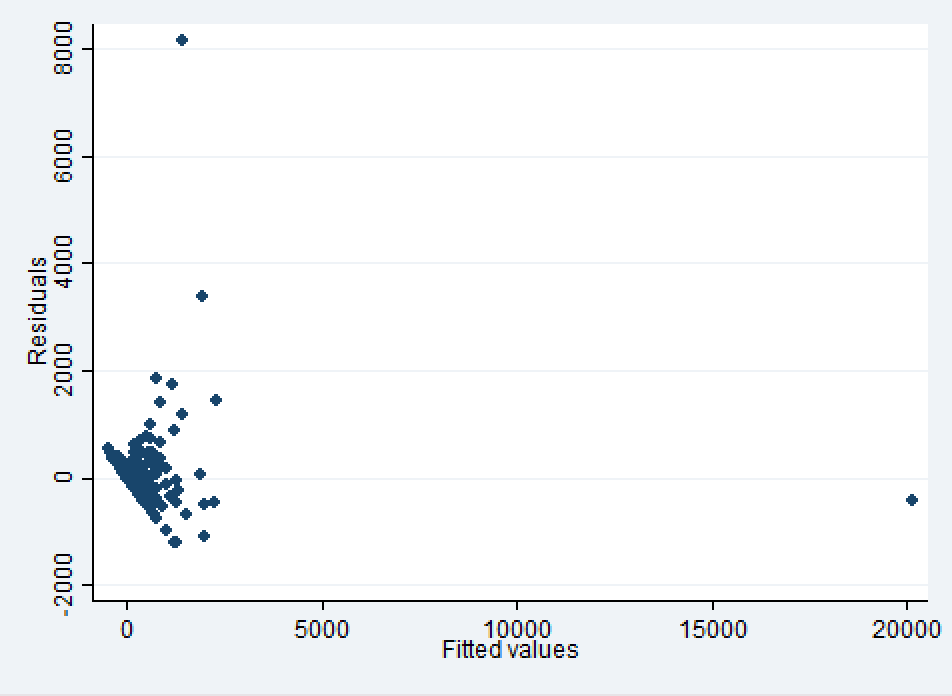
\includegraphics[height=0.3\textheight]{figApp/Model-2-2007-resid}\label{Residuals Plot of OLS Estimation of Model (2) (for Year 2007).}}
\end{minipage}

\begin{minipage}{3.3cm}
    \centering
    \subtop[]{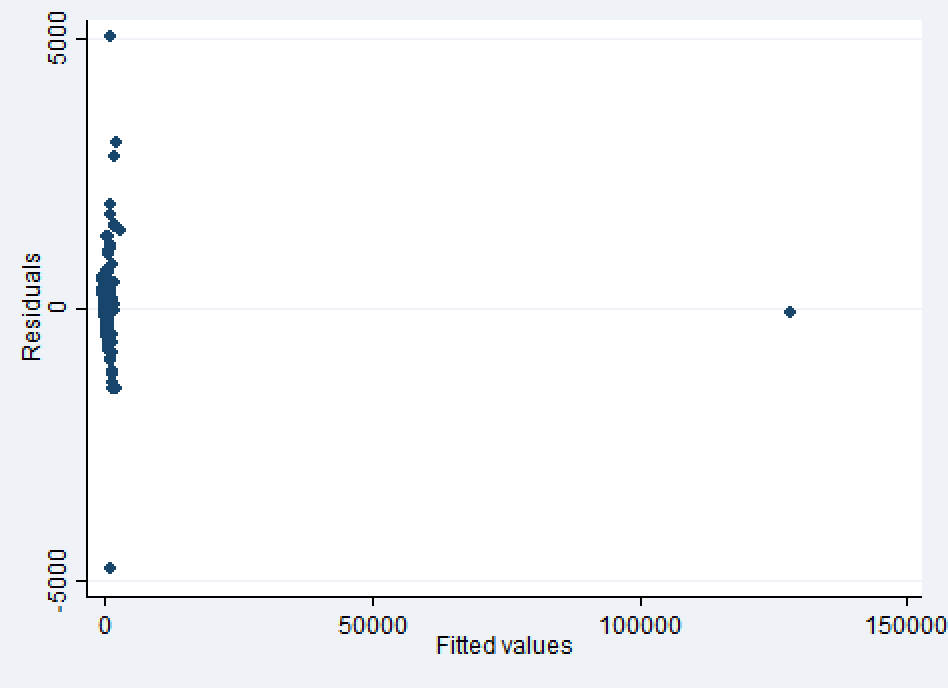
\includegraphics[height=0.3\textheight]{figApp/Model-2-2012-resid}\label{Residuals Plot of OLS Estimation of Model (2) (for Year 2012).}}
\end{minipage}

\mycaption[Time Series Plots in Gross Profits, Total Assets, and Market Concentration.]{(a)~Residuals Plot of OLS Estimation of Model (2) (for Year 2002). (b)~Residuals Plot of OLS Estimation of Model (2) (for Year 2007). (c)~Residuals Plot of OLS Estimation of Model (2) (for Year 2012). }
\label{fig:multiRH02}
\end{figure}

\iffalse
\newpage
\begin{figure}[h]
\centering
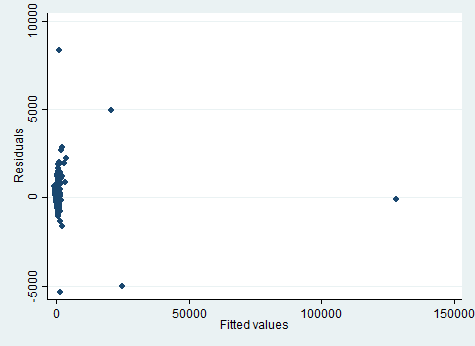
\includegraphics[scale=0.75]{figApp/Residuals_Plot_Model_2}\label{Residuals Plot of OLS Estimation of Model (2)}
\mycaption[Residuals Plot of OLS Estimation of Model (2).]{Residuals Plot of OLS Estimation of Model (2).}
\end{figure}
\fi

\clearpage
\begin{table}[h]
\centering
\begin{tabular}{ c | c }
	\hline
	\textbf{Breusch-Pagan-Godfrey Test for Model (2) (for Year 2002)} \\
    \textbf{Regressand: Squared Residuals} \\
    \hline \hline
    Number of Observations & 213 \\
	\hline
    $R^{2}$ & 0.995 \\
    Adjusted $R^{2}$ & 0.994 \\
    \hline
    $F(41, 171)$ & 878.21 \\
    $Prob > F$ & 0.0000 \\
    \hline \hline
\end{tabular} \\
\mycaption[Breusch-Pagan-Godfrey Test for Model (2) (for Year 2002)]{Bresuch-Pagan Test for Model (2) (for Year 2002)}
\end{table}

\begin{table}[h]
\centering
\begin{tabular}{ c | c }
	\hline
	\textbf{Breusch-Pagan-Godfrey Test for Model (2) (for Year 2007)} \\
    \textbf{Regressand: Squared Residuals} \\
    \hline \hline
    Number of Observations & 245 \\
	\hline
    $R^{2}$ & 0.972 \\
    Adjusted $R^{2}$ & 0.967 \\
    \hline
    $F(40, 204)$ & 179.11 \\
    $Prob > F$ & 0.0000 \\
    \hline \hline
\end{tabular} \\
\mycaption[Breusch-Pagan Test for Model (2) (for Year 2007)]{Bresuch-Pagan Test for Model (2) (for Year 2007)}
\end{table}

\begin{table}[h]
\centering
\begin{tabular}{ c | c }
	\hline
	\textbf{Breusch-Pagan Test for Model (2) (for Year 2012)} \\
    \textbf{Regressand: Squared Residuals} \\
    \hline \hline
    Number of Observations & 240 \\
	\hline
    $R^{2}$ & 0.999 \\
    Adjusted $R^{2}$ & 0.999 \\
    \hline
    $F(40, 199)$ & 5828.45 \\
    $Prob > F$ & 0.0000 \\
    \hline \hline
\end{tabular} \\
\mycaption[Breusch-Pagan Test for Model (2) (for Year 2012)]{Bresuch-Pagan Test for Model (2) (for Year 2012)}
\end{table}

\iffalse
\begin{table}[h]
\centering
\begin{tabular}{ c | c }
	\hline
	\textbf{Breusch-Pagan Test for Model 2} \\
    \textbf{Regressand: Squared Residuals} \\
    \hline \hline
    Number of Observations & 698 \\
	\hline
    $R^{2}$ & 0.974 \\
    Adjusted $R^{2}$ & 0.972 \\
    \hline
    $F(45, 652)$ & 532.02 \\
    $Prob > F$ & 0.0000 \\
    \hline \hline
\end{tabular} \\
\mycaption[Breusch-Pagan Test for Model (2)]{Bresuch-Pagan Test for Model (2)}
\end{table}
\fi

\clearpage
\begin{figure}[h]
\begin{minipage}{3.3cm}
    \centering
    \subtop[]{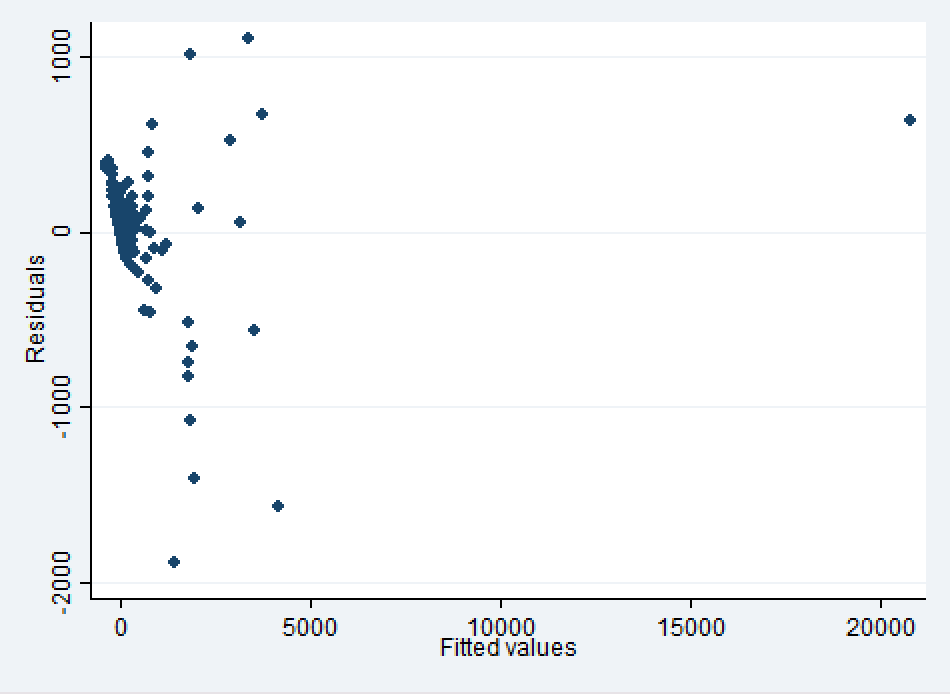
\includegraphics[height=0.3\textheight]{figApp/Model-3-2002-resid}\label{Residuals Plot of OLS Estimation of Model (3) (for Year 2002).}}
\end{minipage}
\hspace{5cm}
\begin{minipage}{3.3cm}
    \centering
    \subtop[]{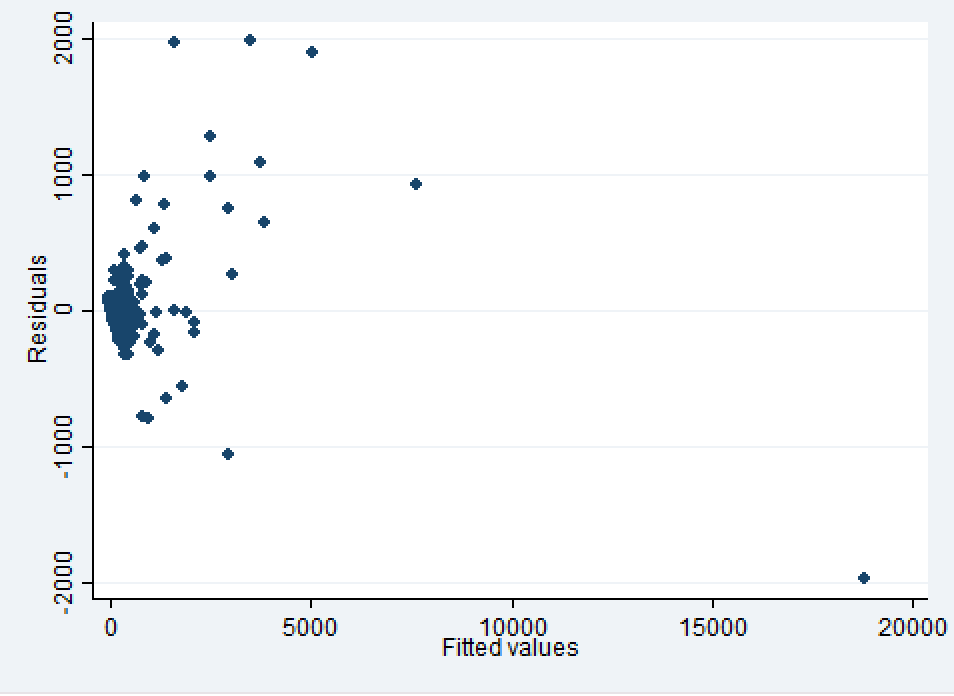
\includegraphics[height=0.3\textheight]{figApp/Model-3-2007-resid}\label{Residuals Plot of OLS Estimation of Model (3) (for Year 2007).}}
\end{minipage}

\begin{minipage}{3.3cm}
    \centering
    \subtop[]{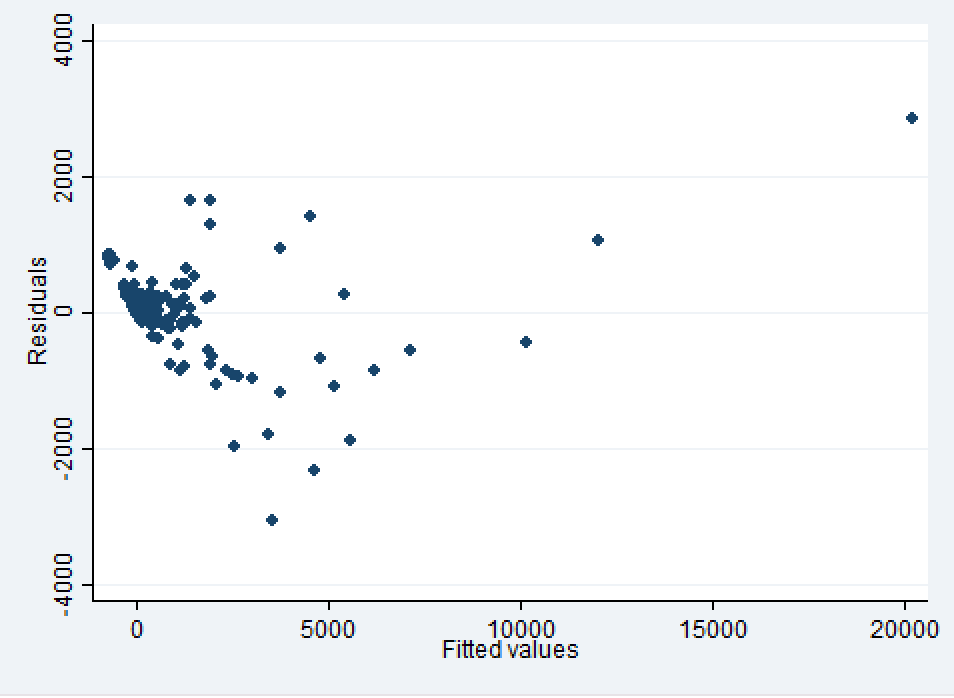
\includegraphics[height=0.3\textheight]{figApp/Model-3-2012-resid}\label{Residuals Plot of OLS Estimation of Model (3) (for Year 2012).}}
\end{minipage}

\mycaption[Time Series Plots in Gross Profits, Total Assets, and Market Concentration.]{(a)~Residuals Plot of OLS Estimation of Model (3) (for Year 2002). (b)~Residuals Plot of OLS Estimation of Model (3) (for Year 2007). (c)~Residuals Plot of OLS Estimation of Model (3) (for Year 2012). }
\label{fig:multiRH02}
\end{figure}

\clearpage
\begin{table}[h]
\centering
\begin{tabular}{ c | c }
	\hline
	\textbf{Breusch-Pagan-Godfrey Test for Model (3) (for Year 2002)} \\
    \textbf{Regressand: Squared Residuals} \\
    \hline \hline
    Number of Observations & 341 \\
	\hline
    $R^{2}$ & 0.858 \\
    Adjusted $R^{2}$ & 0.848 \\
    \hline
    $F(22, 318)$ & 87.14 \\
    $Prob > F$ & 0.0000 \\
    \hline \hline
\end{tabular} \\
\mycaption[Breusch-Pagan-Godfrey Test for Model (3) (for Year 2002)]{Bresuch-Pagan Test for Model (3) (for Year 2002)}
\end{table}

\begin{table}[h]
\centering
\begin{tabular}{ c | c }
	\hline
	\textbf{Breusch-Pagan-Godfrey Test for Model (3) (for Year 2007)} \\
    \textbf{Regressand: Squared Residuals} \\
    \hline \hline
    Number of Observations & 279 \\
	\hline
    $R^{2}$ & 0.834 \\
    Adjusted $R^{2}$ & 0.818 \\
    \hline
    $F(22, 256)$ & 57.83 \\
    $Prob > F$ & 0.0000 \\
    \hline \hline
\end{tabular} \\
\mycaption[Breusch-Pagan Test for Model (3) (for Year 2007)]{Bresuch-Pagan Test for Model (3) (for Year 2007)}
\end{table}

\begin{table}[h]
\centering
\begin{tabular}{ c | c }
	\hline
	\textbf{Breusch-Pagan Test for Model (3) (for Year 2012)} \\
    \textbf{Regressand: Squared Residuals} \\
    \hline \hline
    Number of Observations & 282 \\
	\hline
    $R^{2}$ & 0.775 \\
    Adjusted $R^{2}$ & 0.756 \\
    \hline
    $F(22, 259)$ & 40.50 \\
    $Prob > F$ & 0.0000 \\
    \hline \hline
\end{tabular} \\
\mycaption[Breusch-Pagan Test for Model (3) (for Year 2012)]{Bresuch-Pagan Test for Model (3) (for Year 2012)}
\end{table}

\newpage
\begin{table}[h]
\begin{tabular}{ c | c }
	\hline
	\textbf{Model (2) (for Year 2002) with White Robust Standard Errors} \\
    \textbf{Non-Manufacturing Industries} \\
    \textbf{Regressand: Gross Profits} \\
    \hline \hline
    Number of Observations & 213 \\
	\hline
    $R^{2}$ & 0.975 \\
    Adjusted $R^{2}$ & 0.969 \\
    \hline
    $F(36, 171)$ & $5.4 \times 10^{12}$ \\
    $Prob > F$ & 0.0000 \\
    \hline \hline
\end{tabular} \\

\begin{tabular}{ l | c | c | c | c | c }
	\hline
	\textbf{Regressors} & \textbf{Estimators} & \textbf{Std. Errors} & $t$ & $P > |t|$ & 95\% CI \\
    & $\hat{\beta}$ & $\hat{\sigma}$ & & & \\
    \hline \hline
	Total Assets & 0.0581 & 0.000267 & 217.29 & 0.000 & (0.0575, 0.0585) \\
	\hline
    Per Cent of Revenue Held & 4.859 & 2.127 & 2.28 & 0.024 & (0.660, 9.058) \\
    By Industry’s Top 50 Firms & & & & & \\
    \hline
    \hline \hline
\end{tabular}
\mycaption[OLS Estimation of Model (2) (for Year 2002) with White Robust Standard Errors: Coefficients for Main Regressors, Controlling for Year and Industry Fixed Effects (Not Shown)]{OLS Estimation of Model (2) (for Year 2002) with White Robust Standard Errors: Coefficients for Main Regressors, Controlling for Industry Fixed Effects (Not Shown)}
\end{table}

\begin{table}[h]
\begin{tabular}{ c | c }
	\hline
	\textbf{Model (2) (for Year 2007) (with White Robust Standard Errors)} \\
    \textbf{Non-Manufacturing Industries} \\
    \textbf{Regressand: Gross Profits} \\
    \hline \hline
    Number of Observations & 245 \\
	\hline
    $R^{2}$ & 0.789 \\
    Adjusted $R^{2}$ & 0.747 \\
    \hline
    $F(37, 204)$ & $4.1 \times 10^{11}$ \\
    $Prob > F$ & 0.0000 \\
    \hline \hline
\end{tabular} \\

\begin{tabular}{ l | c | c | c | c | c }
	\hline
	\textbf{Regressors} & \textbf{Estimators} & \textbf{Std. Errors} & $t$ & $P > |t|$ & 95\% CI \\
    & $\hat{\beta}$ & $\hat{\sigma}$ & & & \\
    \hline \hline
	Total Assets & 0.0447 & 0.00137 & 32.65 & 0.000 & (0.0420, 0.0474) \\
	\hline
    Per Cent of Revenue Held & 8.864 & 2.790 & 3.18 & 0.002 & (3.362, 14.365) \\
    By Industry’s Top 50 Firms & & & & & \\
    \hline
    \hline \hline
\end{tabular}
\mycaption[OLS Estimation of Model (2) (for Year 2007) with White Robust Standard Errors: Coefficients for Main Regressors, Controlling for Year and Industry Fixed Effects (Not Shown)]{OLS Estimation of Model (2) (for Year 2007) with White Robust Standard Errors: Coefficients for Main Regressors, Controlling for Industry Fixed Effects (Not Shown)}
\end{table}

\begin{table}[h]
\begin{tabular}{ c | c }
	\hline
	\textbf{Model (2) (for Year 2012) with White Robust Standard Errors} \\
    \textbf{Non-Manufacturing Industries} \\
    \textbf{Regressand: Gross Profits} \\
    \hline \hline
    Number of Observations & 240 \\
	\hline
    $R^{2}$ & 0.993 \\
    Adjusted $R^{2}$ & 0.991 \\
    \hline
    $F(36, 199)$ & $1.0 \times 10^{6}$ \\
    $Prob > F$ & 0.0000 \\
    \hline \hline
\end{tabular} \\

\begin{tabular}{ l | c | c | c | c | c }
	\hline
	\textbf{Regressors} & \textbf{Estimators} & \textbf{Std. Errors} & $t$ & $P > |t|$ & 95\% CI \\
    & $\hat{\beta}$ & $\hat{\sigma}$ & & & \\
    \hline \hline
	Total Assets & 0.0398 & 0.000161 & 247.02 & 0.000 & (0.0395, 0.0401) \\
	\hline
    Per Cent of Revenue Held & 7.230 & 3.498 & 2.07 & 0.040 & (0.331, 14.128) \\
    By Industry’s Top 50 Firms & & & & & \\
    \hline
    \hline \hline
\end{tabular}
\mycaption[OLS Estimation of Model (2) (for Year 2012) with White Robust Standard Errors: Coefficients for Main Regressors, Controlling for Year and Industry Fixed Effects (Not Shown)]{OLS Estimation of Model (2) (for Year 2012) with White Robust Standard Errors: Coefficients for Main Regressors, Controlling for Industry Fixed Effects (Not Shown)}
\end{table}

\clearpage
\begin{figure}[h]
\begin{minipage}{3.3cm}
    \centering
    \subtop[]{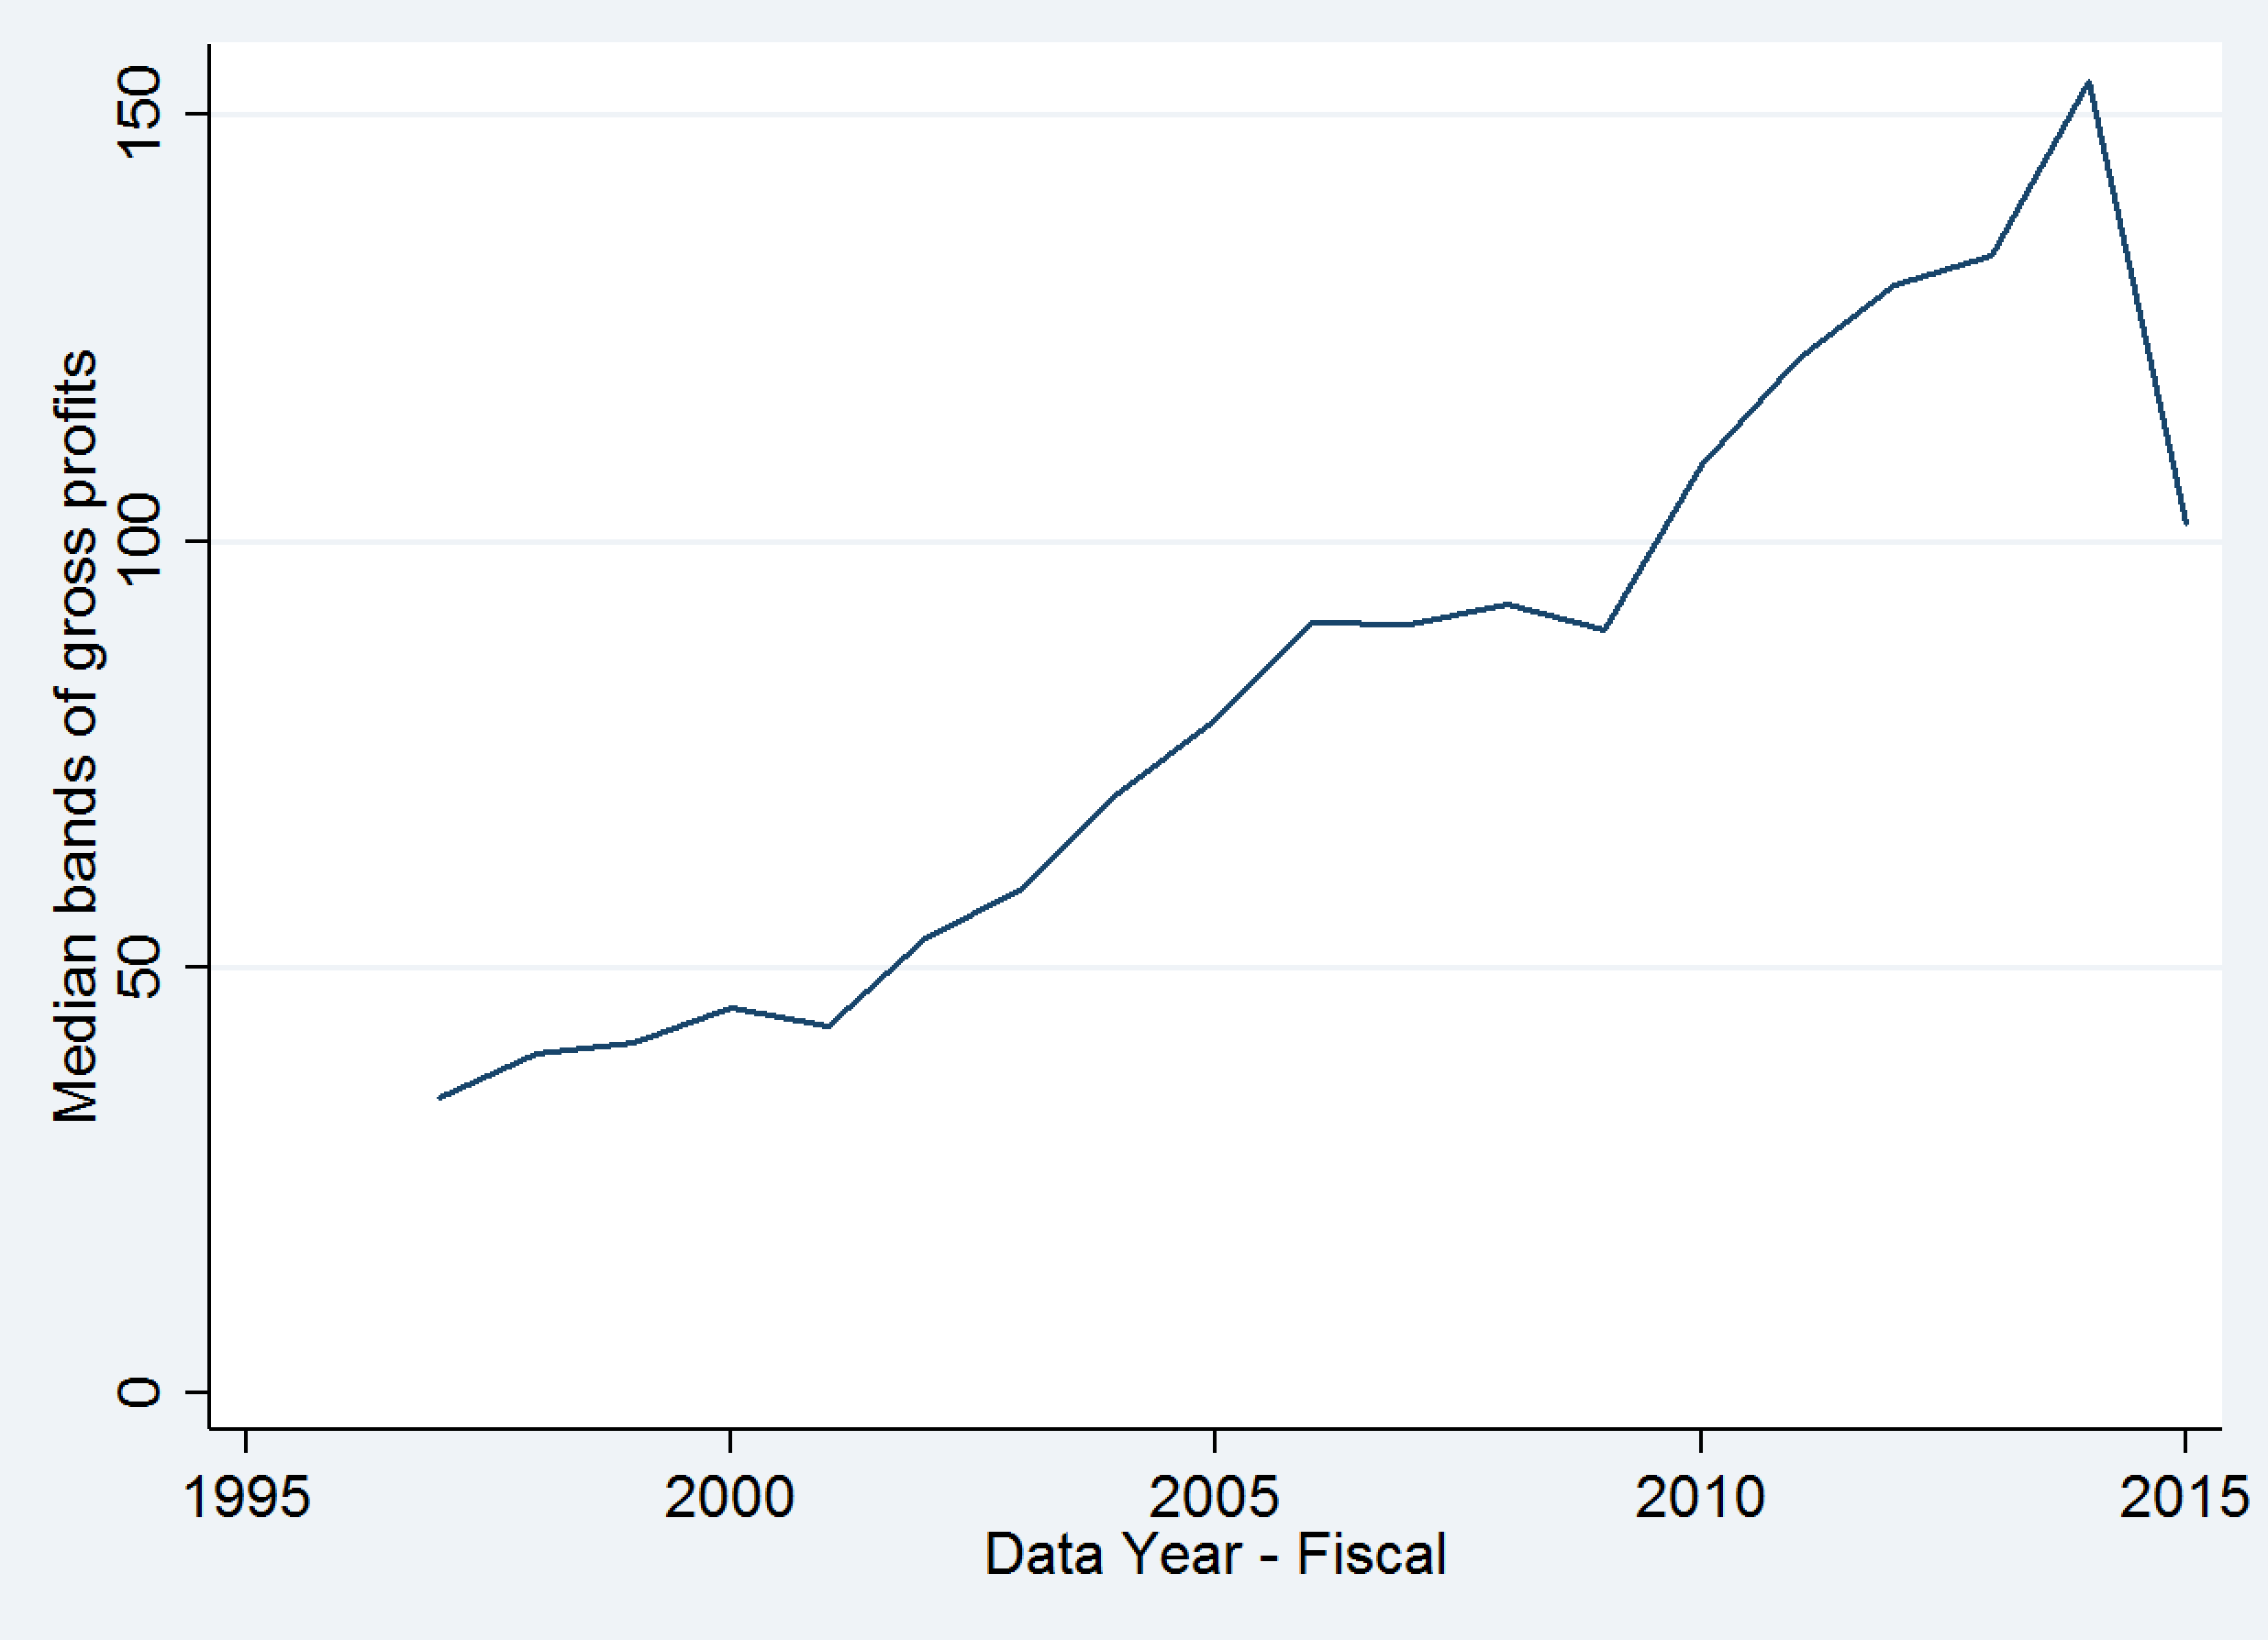
\includegraphics[height=0.3\textheight]{figApp/gp-graph}\label{Time series plot of median gross profits.}}
\end{minipage}
\hspace{5cm}
\begin{minipage}{3.3cm}
    \centering
    \subtop[]{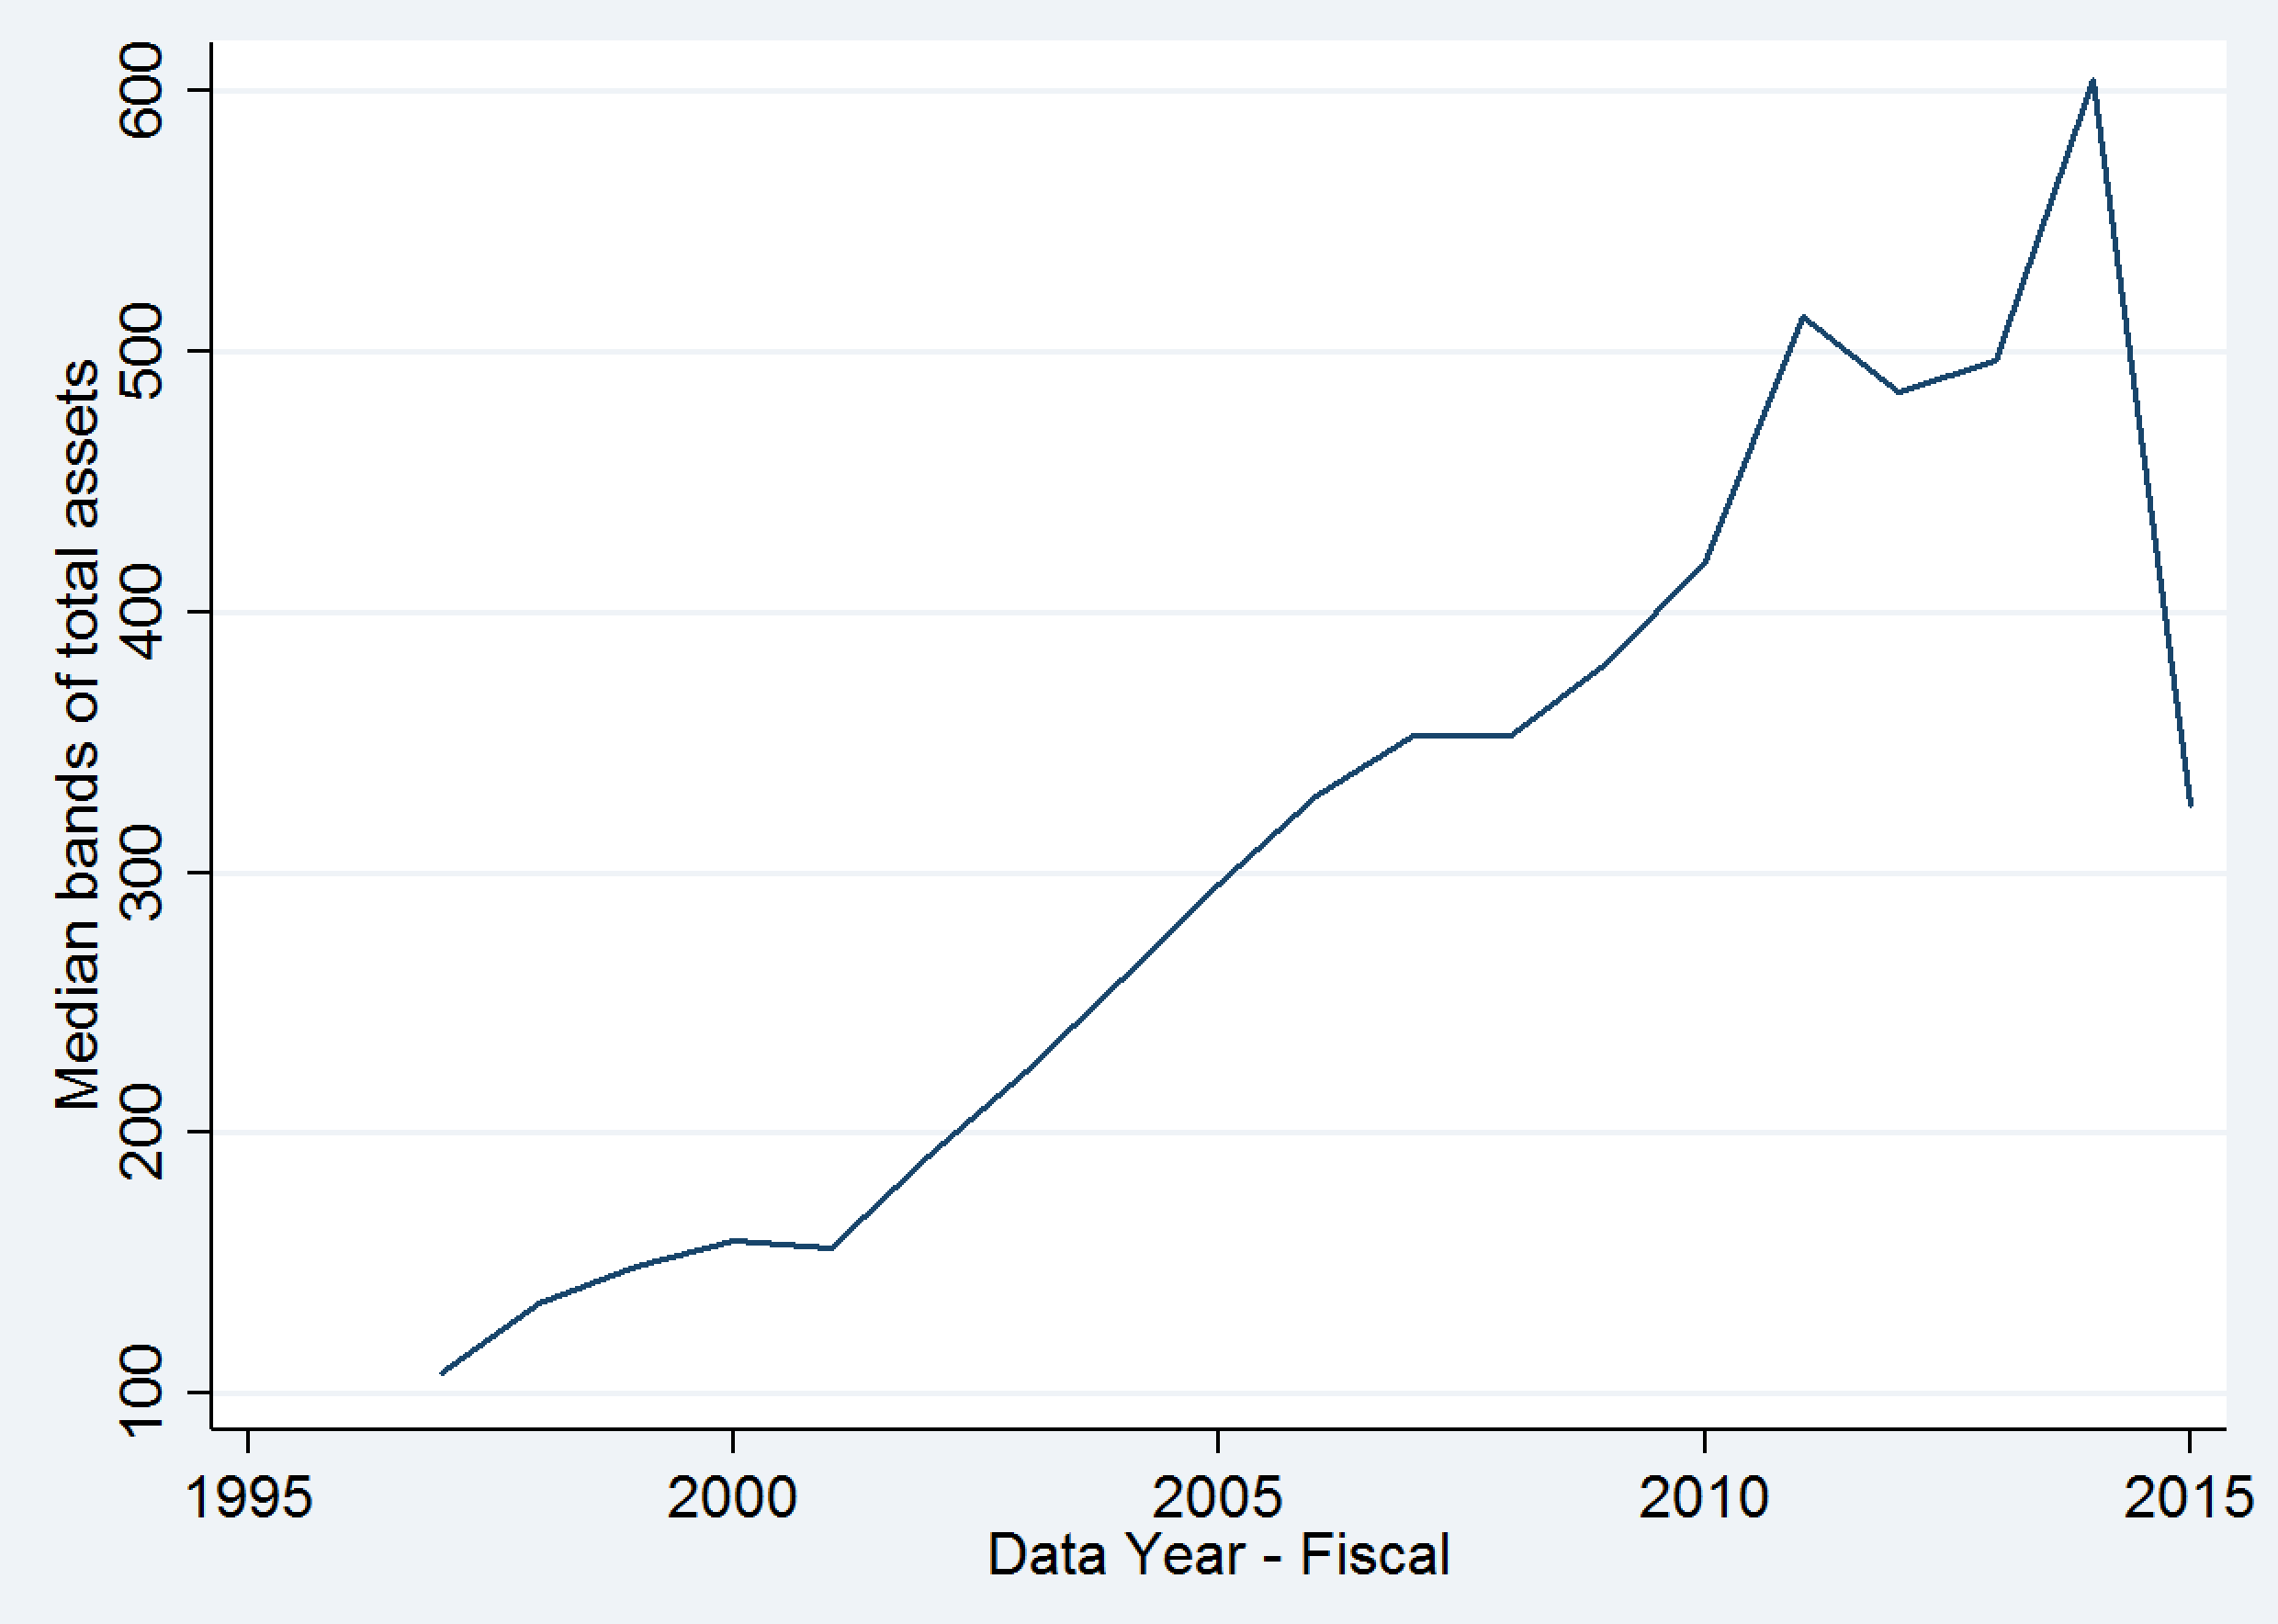
\includegraphics[height=0.3\textheight]{figApp/at-graph}\label{Time series plot of median total assets.}}
\end{minipage}

\begin{minipage}{3.3cm}
    \centering
    \subtop[]{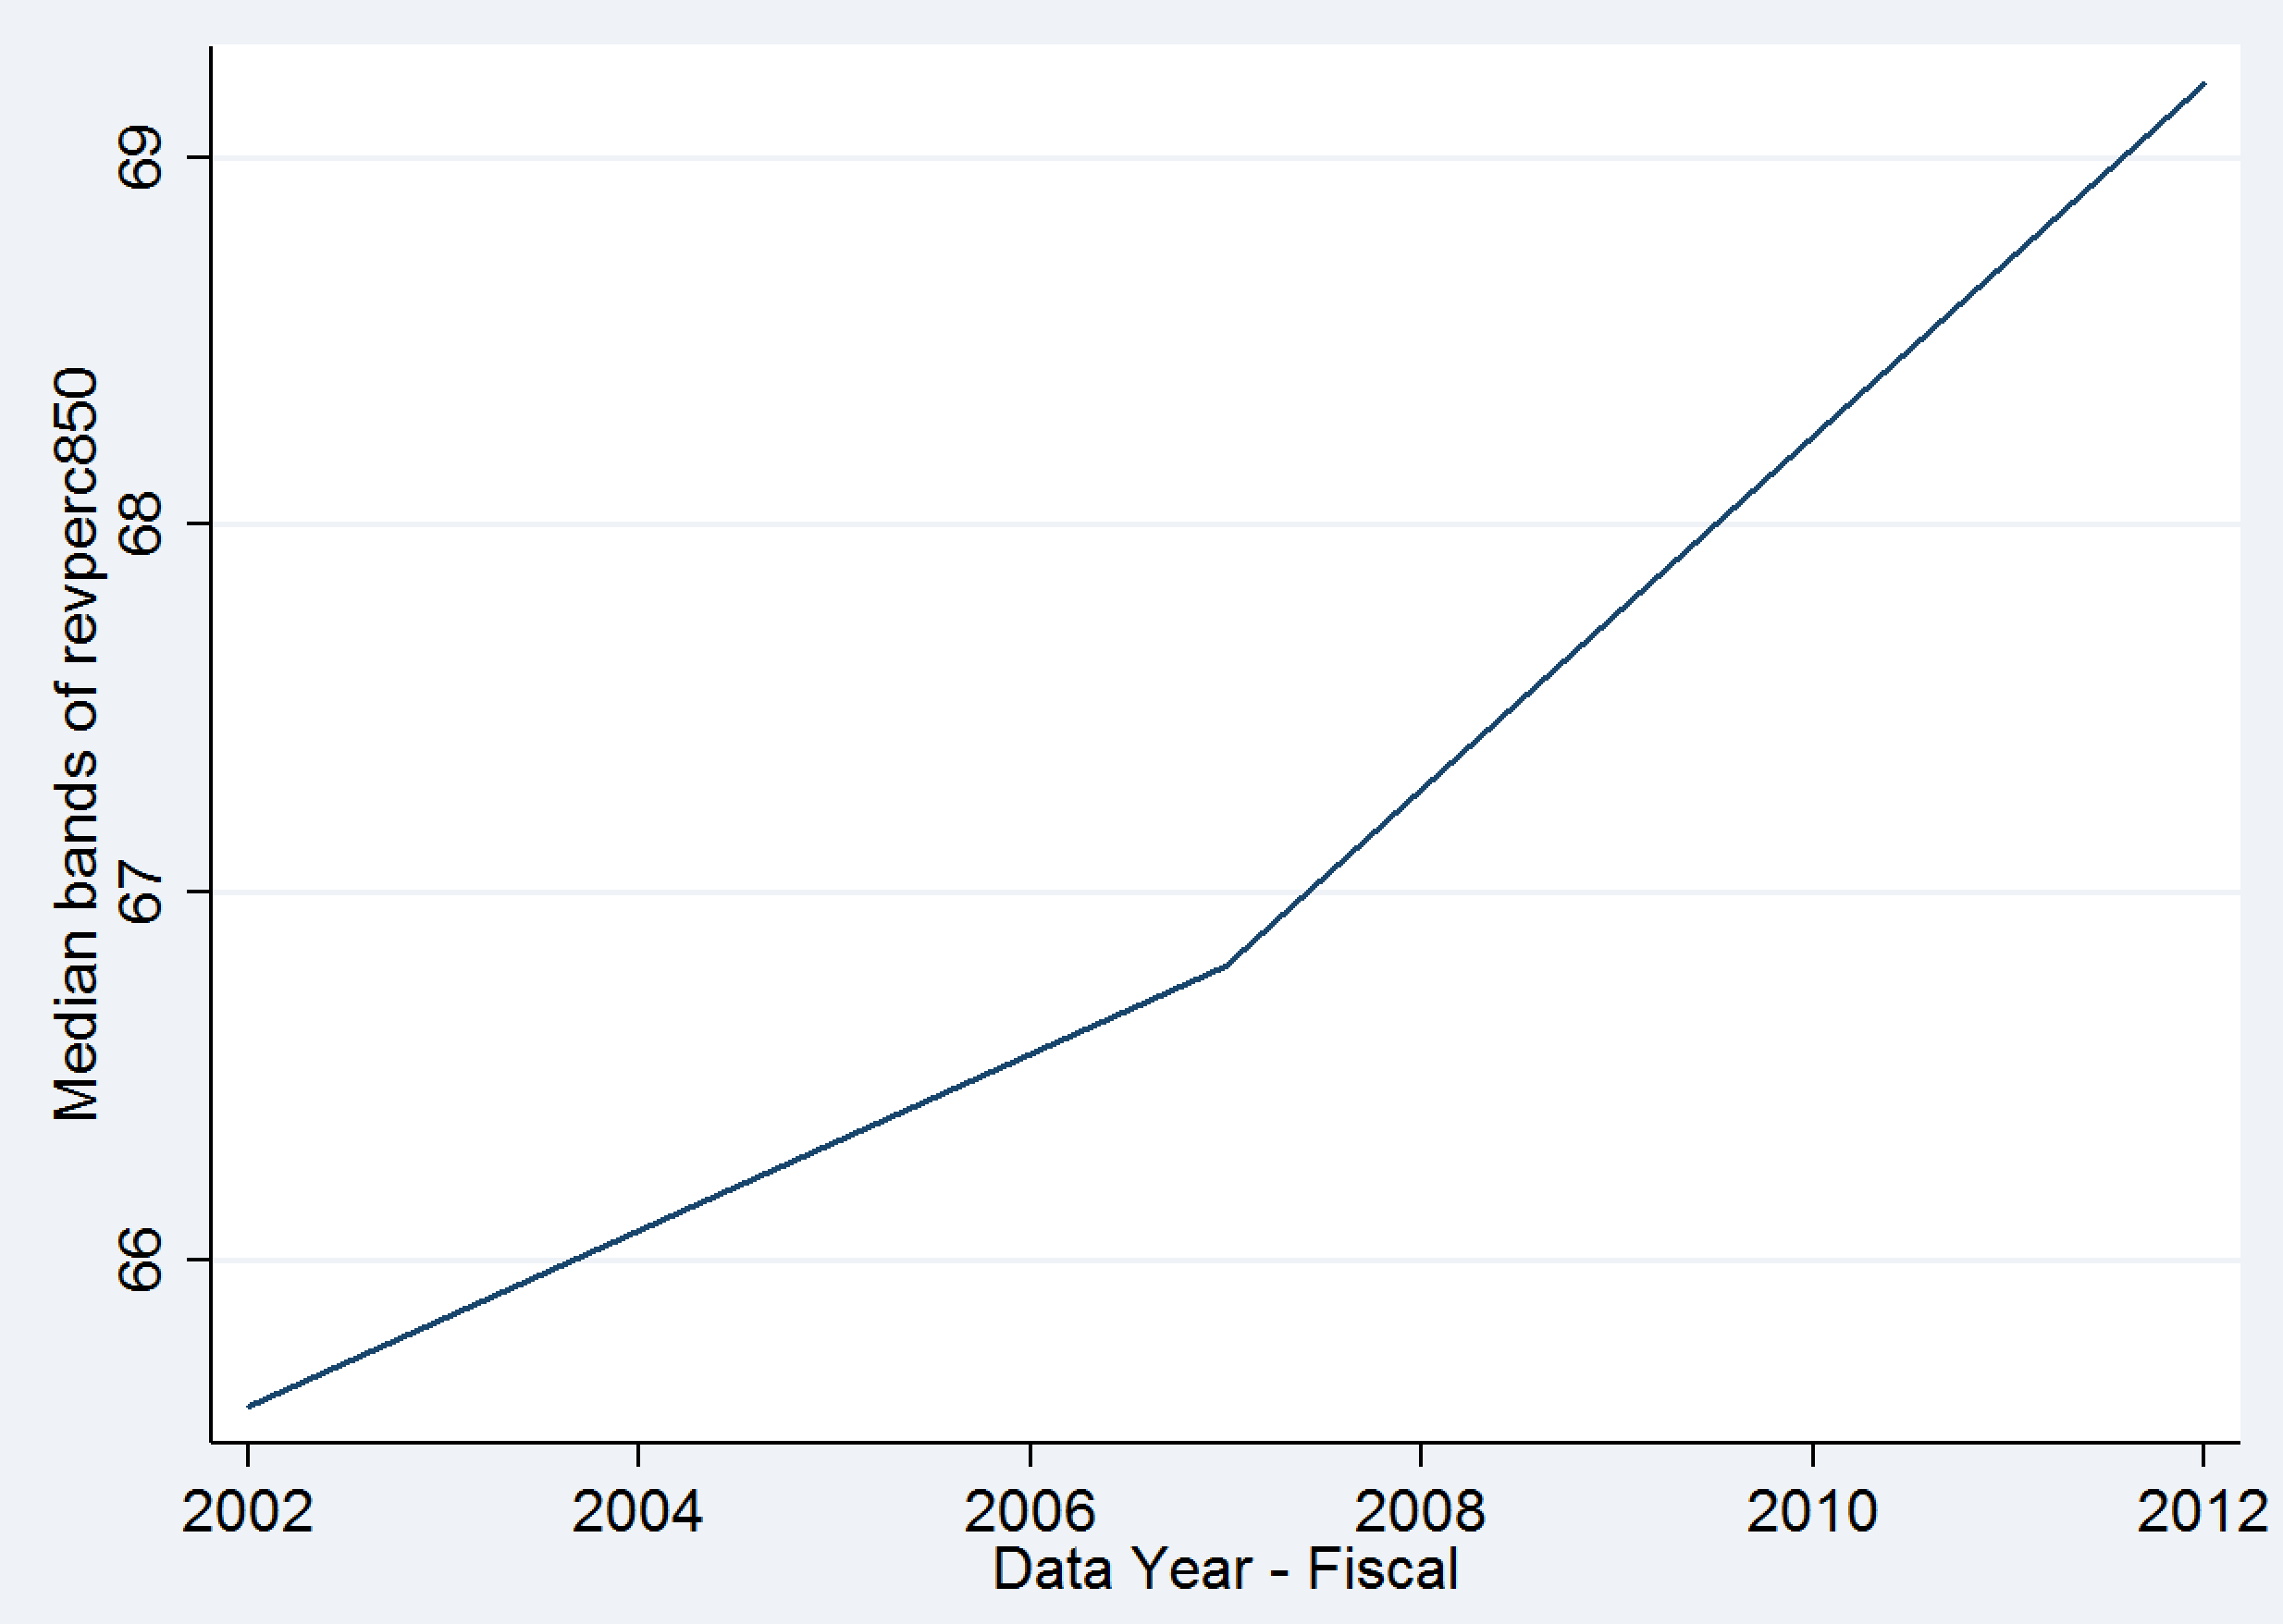
\includegraphics[height=0.3\textheight]{figApp/revperc850-graph}\label{Time series plot of median per cent of revenue held by an industry's top 50 firms.}}
\end{minipage}

\mycaption[Time Series Plots in Gross Profits, Total Assets, and Market Concentration.]{(a)~Time series plot of median gross profits. (b)~Time series plot of median total assets. (c)~Time series plot of median logged gross profits. }
\label{fig:multiRH02}
\end{figure}

\begin{figure}[h]
\begin{minipage}{3.3cm}
    \centering
    \subtop[]{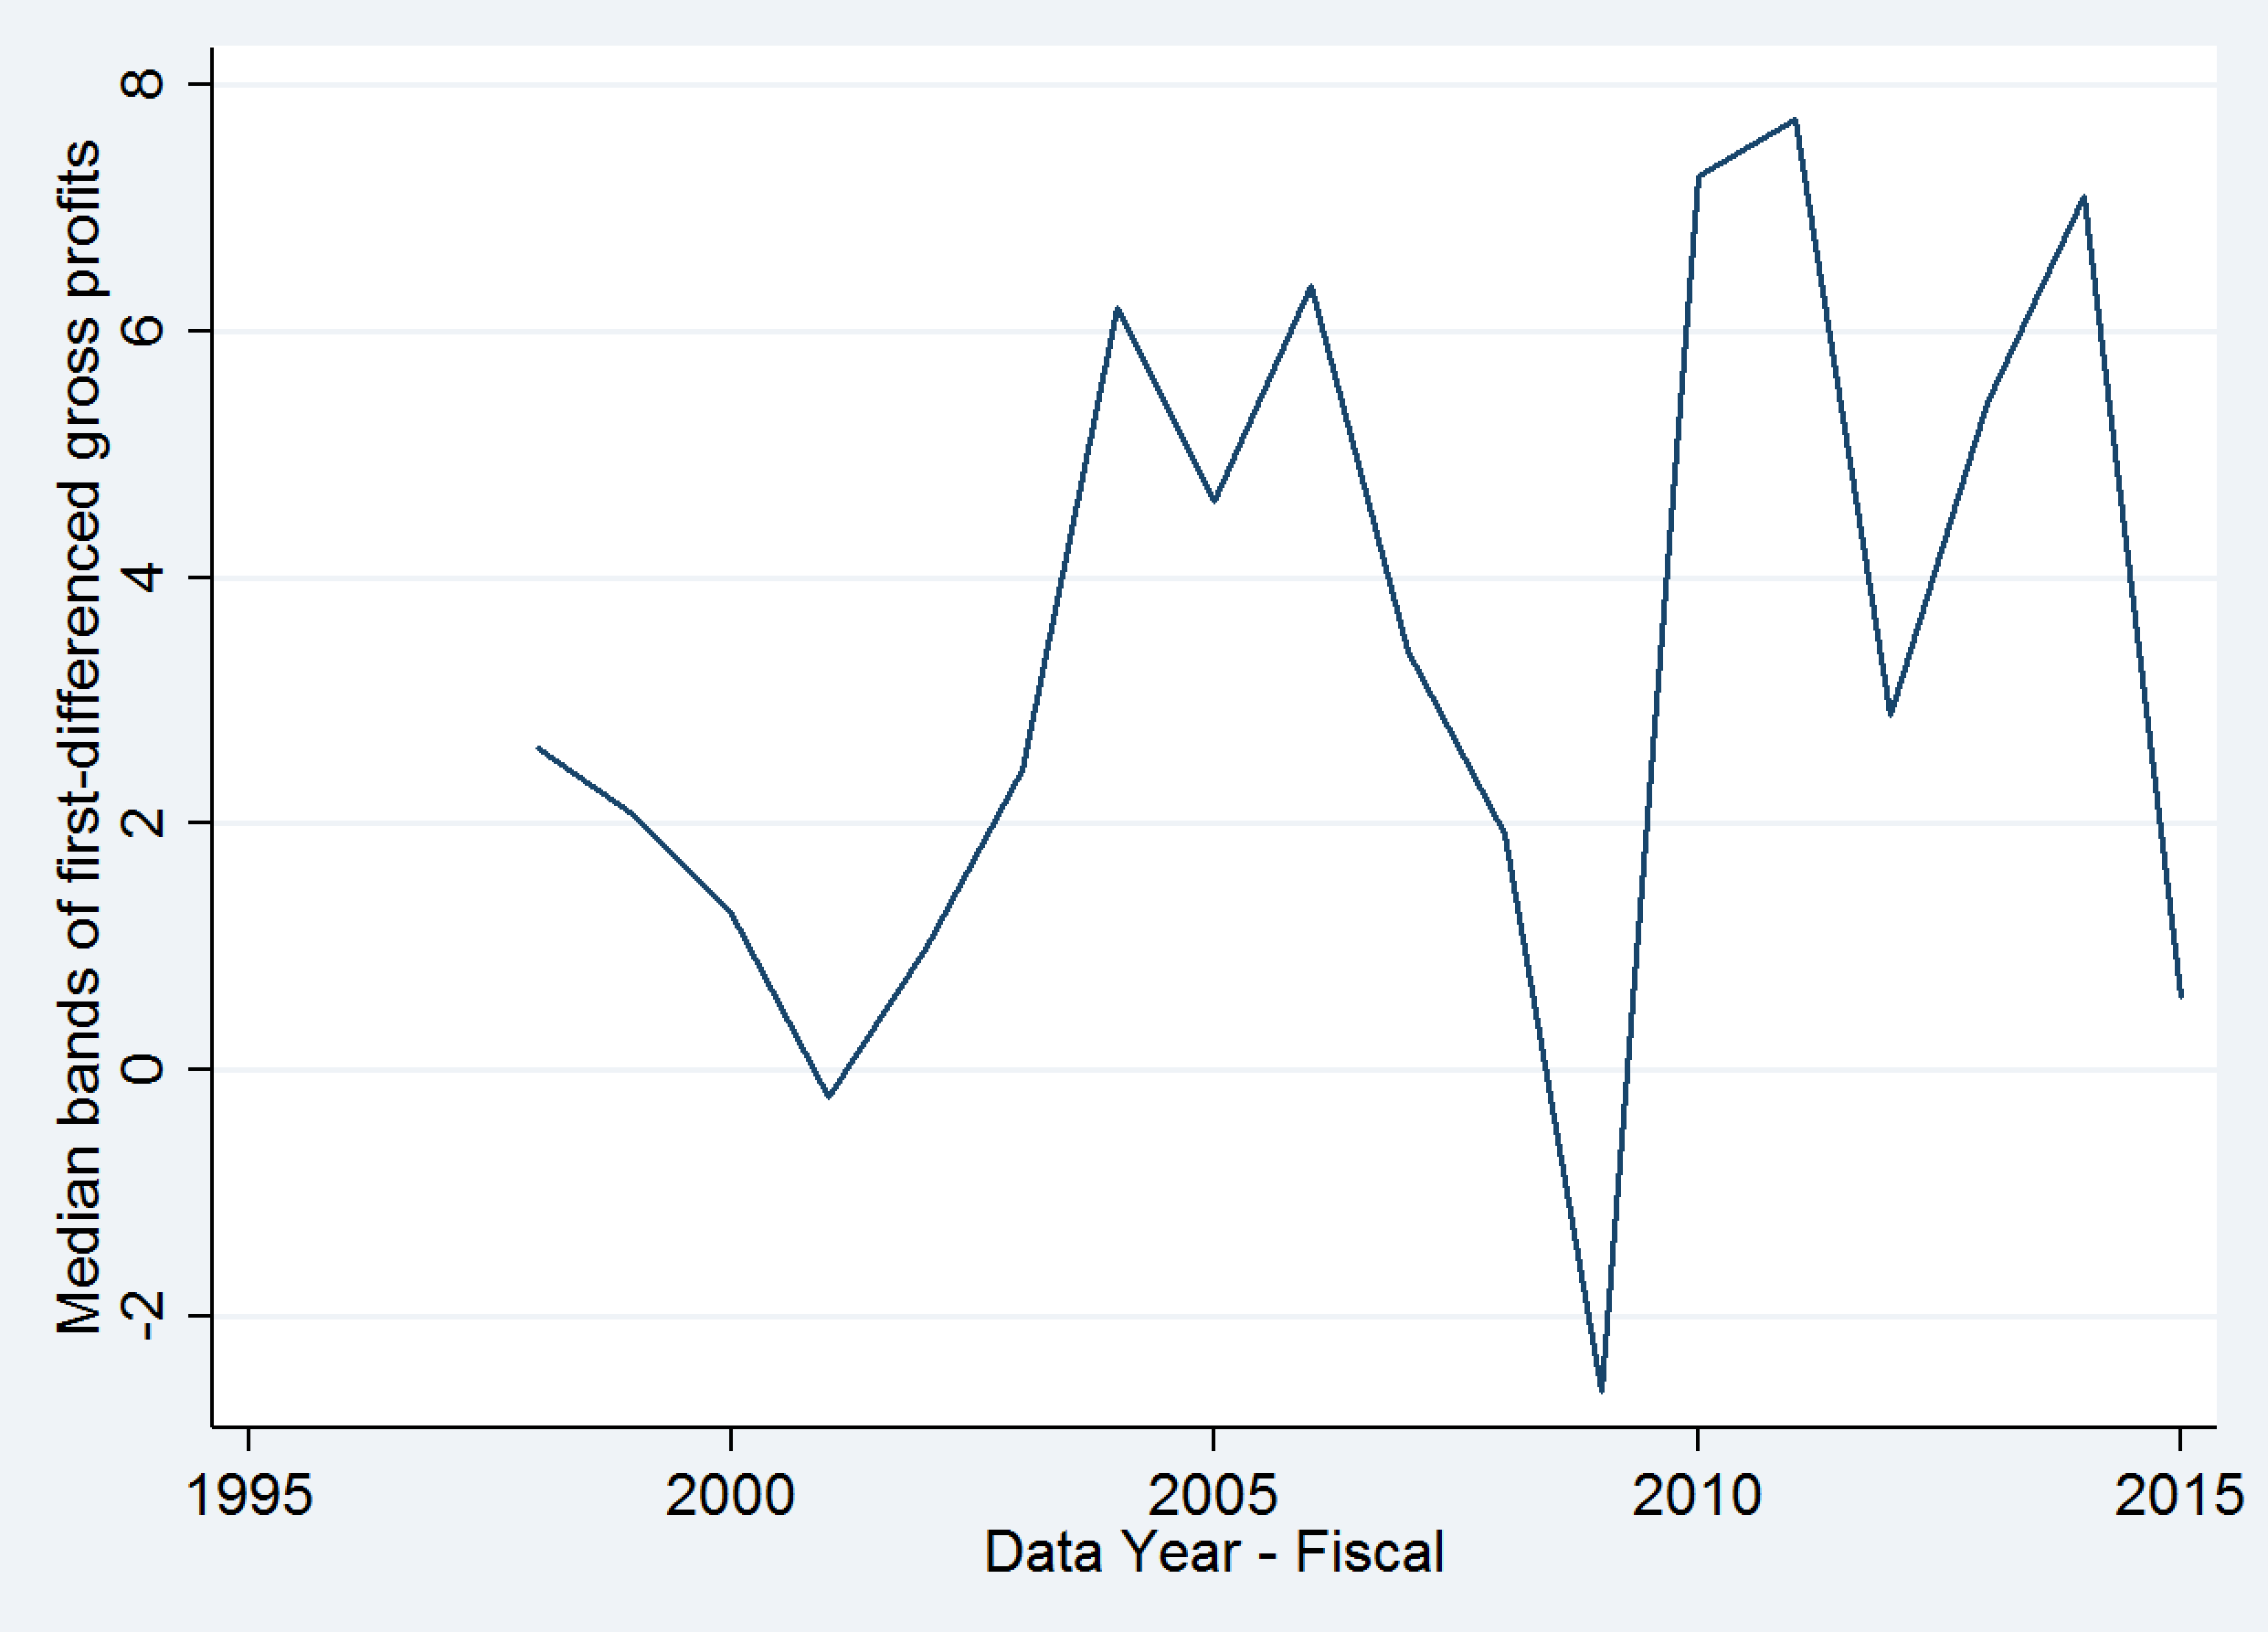
\includegraphics[height=0.3\textheight]{figApp/dgp-graph}\label{Time series plot of median first-differenced gross profits.}}
\end{minipage}
\hspace{5cm}
\begin{minipage}{3.3cm}
    \centering
    \subtop[]{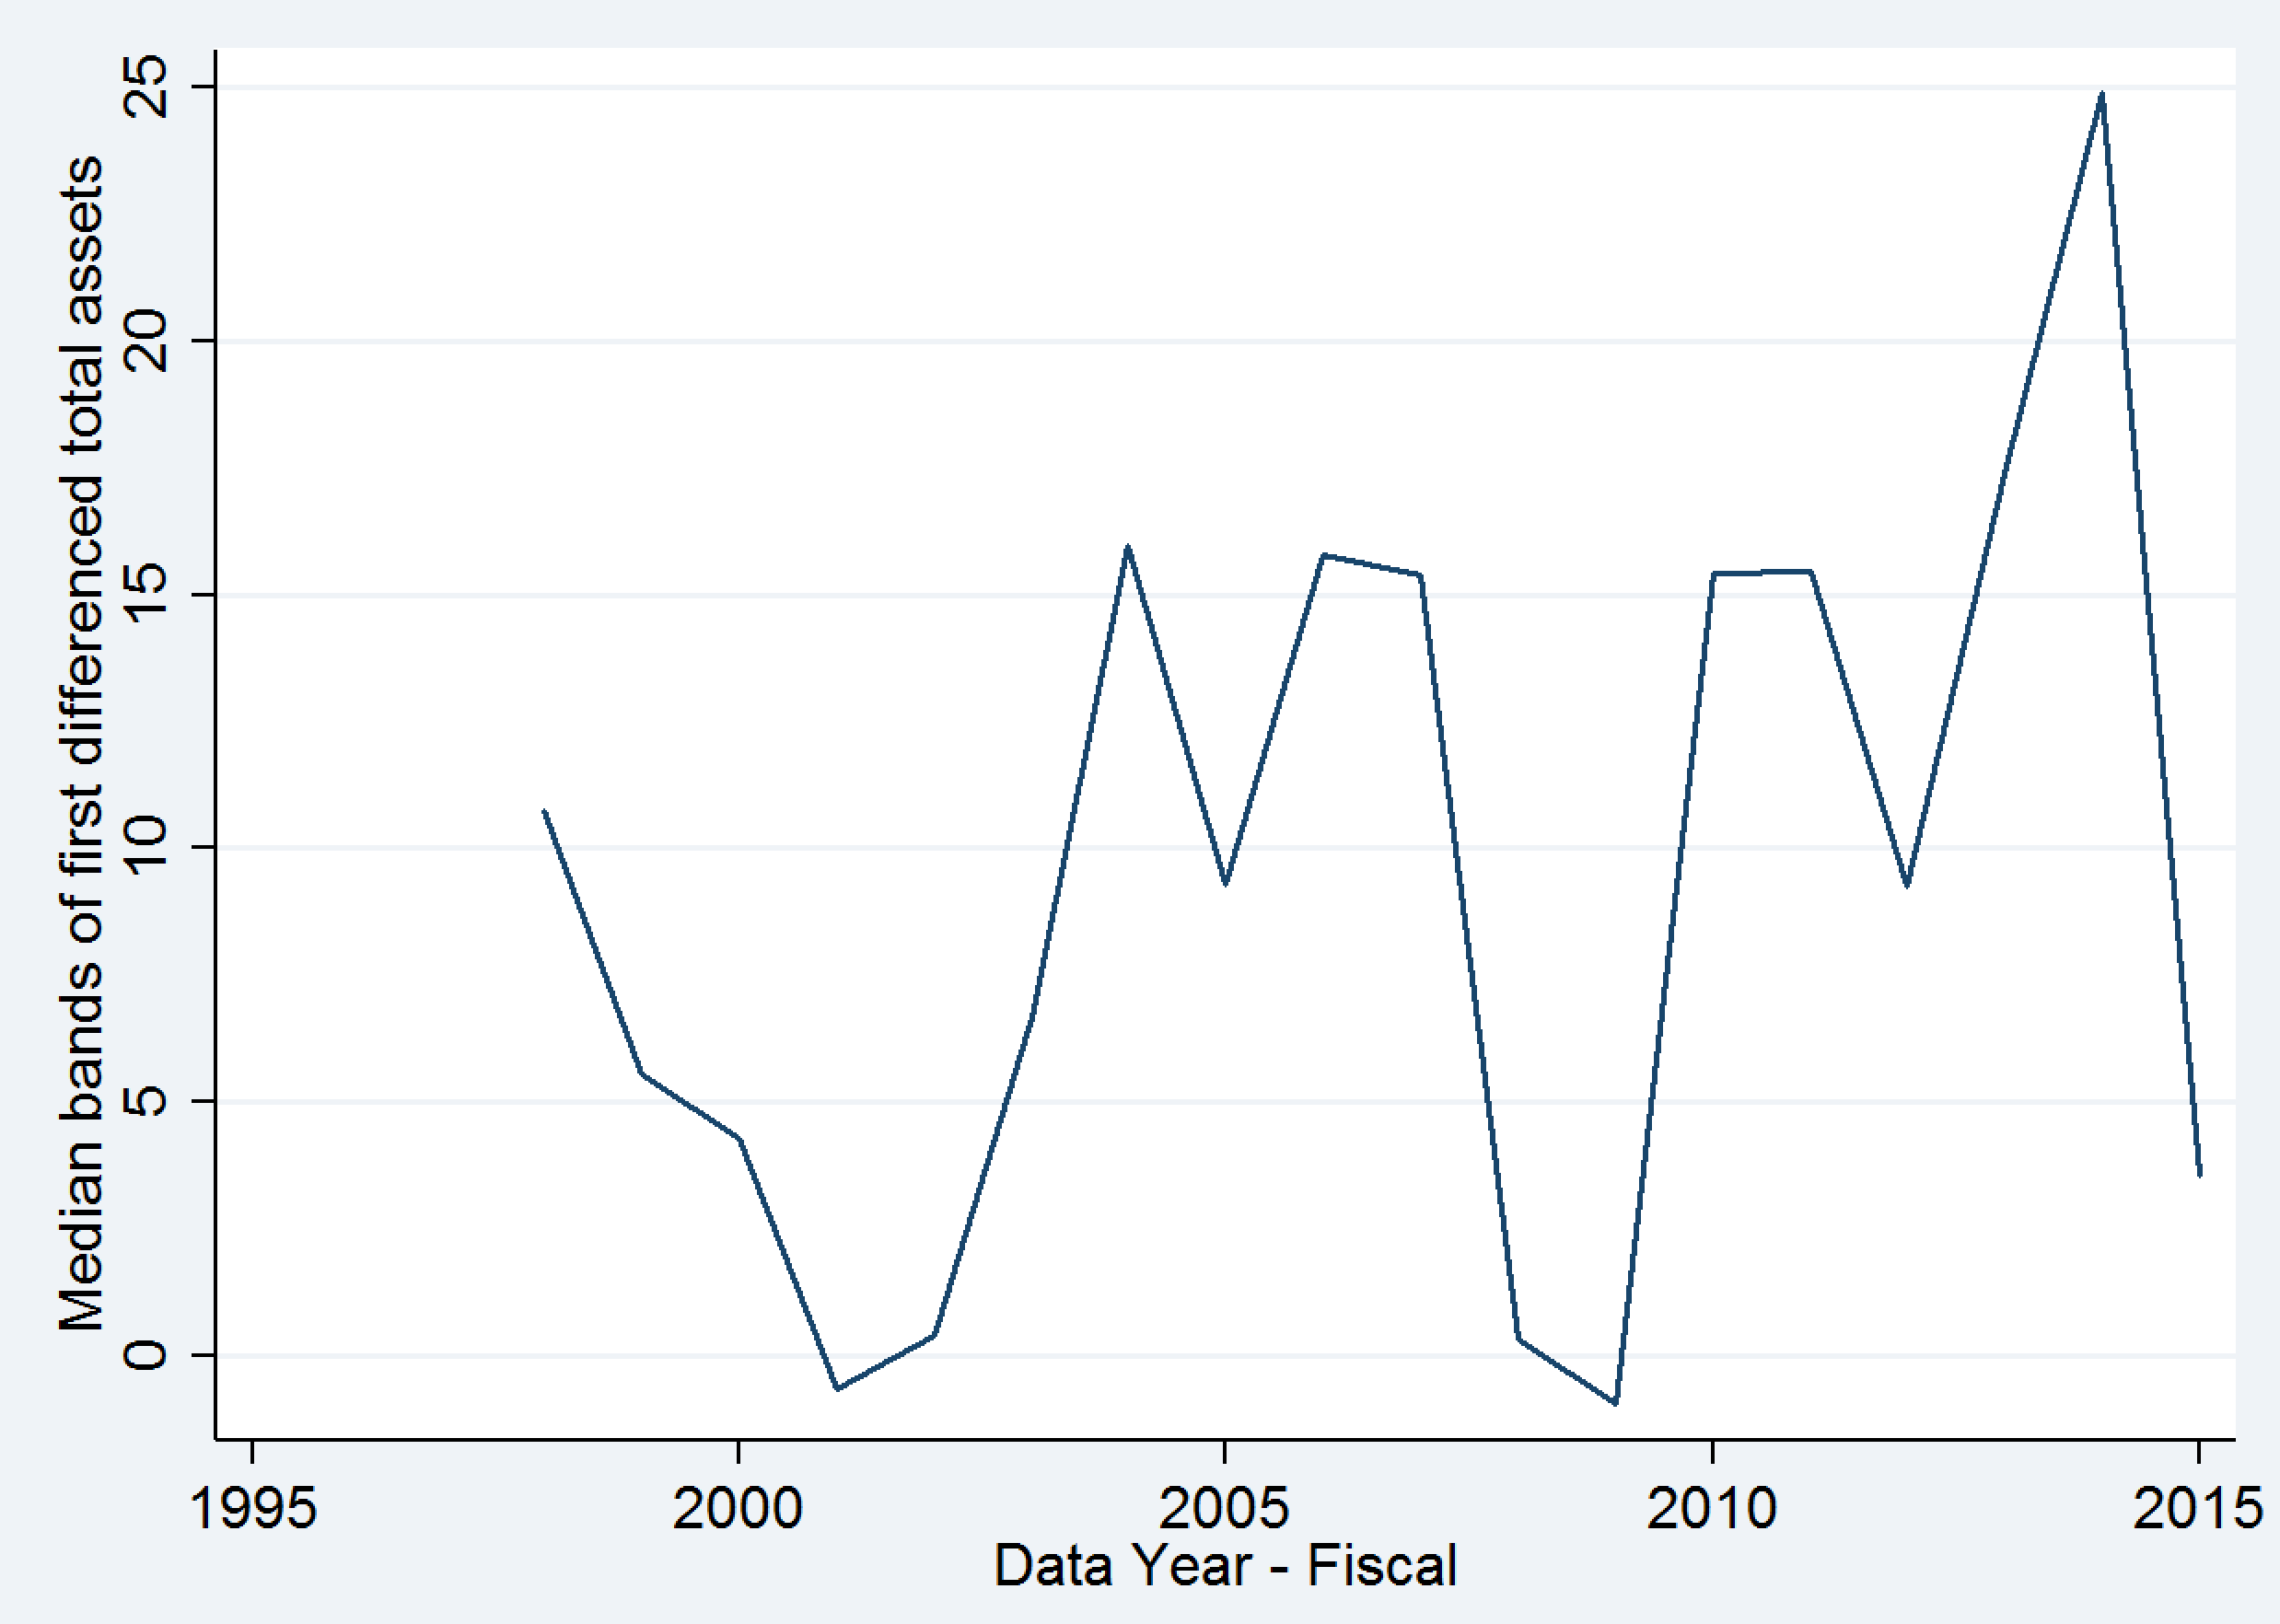
\includegraphics[height=0.3\textheight]{figApp/dat-graph}\label{Time series plot of median first-differenced total assets.}}
\end{minipage}

\mycaption[Time Series Plots in First-Differenced Gross Profits and Total Assets.]{(a)~Time series plot of median first-differenced gross profits. (b)~Time series plot of median first-differenced total assets. }
\label{fig:multiRH02}
\end{figure}
\begin{comment}
\begin{table}[h]
\begin{tabular}{ c | c }
	\hline
	\textbf{Model 2 (Long Run Interpretation By Cointegration)} \\
    \textbf{Non-Manufacturing Industries} \\
    \textbf{Regressand: Gross Profits} \\
    \hline \hline
    Number of Observations & 698 \\
	\hline
    $R^{2}$ & 0.981 \\
    Adjusted $R^{2}$ & 0.980 \\
    \hline
    $F(45, 652)$ & 745.84 \\
    $Prob > F$ & 0.0000 \\
    \hline \hline
\end{tabular} \\

\begin{tabular}{ l | c }
	\hline
	\textbf{Regressors} & \textbf{Estimators} \\
    & $\hat{\beta}$ \\
    \hline \hline
	Total Assets & 0.0401 \\
	\hline
    Per Cent of Revenue Held & 8.327 \\
    By Industry’s Top 50 Firms & \\
    \hline
    \hline \hline
\end{tabular}
\mycaption[Long Run Interpretation of OLS Estimation of Model (2): Coefficients for Main Regressors, Controlling for Year and Industry Fixed Effects (Not Shown)]{Long Run Interpretation of OLS Estimation of Model (2): Coefficients for Main Regressors, Controlling for Year and Industry Fixed Effects (Not Shown)}
\end{table}


\begin{table}[h]
\begin{tabular}{ c | c }
	\hline
	\textbf{Model 3 (Long Run Interpretation By Cointegration)} \\
    \textbf{Manufacturing Industries} \\
    \textbf{Regressand: Gross Profits} \\
    \hline \hline
    Number of Observations & 901 \\
	\hline
    $R^{2}$ & 0.926 \\
    Adjusted $R^{2}$ & 0.924 \\
    \hline
    $F(24, 876)$ & 45.54 \\
    $Prob > F$ & 0.0000 \\
    \hline \hline
\end{tabular} \\

\begin{tabular}{ l | c }
	\hline
	\textbf{Regressors} & \textbf{Estimators} \\
    & $\hat{\beta}$ \\
    \hline \hline
	Total Assets & 0.255 \\
	\hline
    Per Cent of Value Added & 0.600  \\
    By Industry’s Top 50 Firms & \\
    \hline
    \hline \hline
\end{tabular}
\mycaption[Long Run Interpretation of OLS Estimation of Model (3): Coefficients for Main Regressors, Controlling for Year and Industry Fixed Effects (Not Shown)]{Long Run Interpretation of OLS Estimation of Model (3): Coefficients for Main Regressors, Controlling for Year and Industry Fixed Effects (Not Shown)}
\end{table}

\end{comment}
\begin{table}[h]
\begin{tabular}{ c | c }
	\hline
	\textbf{Model (3)} \\
    \textbf{Regressand: Capital Expenditures} \\
    \hline \hline
    Number of Observations & 296,000 \\
	\hline
    $R^{2}$ & 0.915 \\
    Adjusted $R^{2}$ & 0.915 \\
    \hline
    $F(167, 295,832)$ & 19,066.78 \\
    $Prob > F$ & 0.0000 \\
    \hline \hline
\end{tabular} \\

\begin{tabular}{ l | c | c | c | c | c }
	\hline
	\textbf{Regressors} & \textbf{Estimators} & \textbf{Std. Errors} & $t$ & $P > |t|$ & 95\% CI \\
    & $\hat{\beta}$ & $\hat{\sigma}$ & & & \\
    \hline \hline
	Gross Profits & 0.0317 & 0.000285  & 111.48 & 0.000 & (0.0312, 0.0323) \\
	\hline
    Total Assets & -0.000421 & 0.0000184 & -22.86 & 0.000 & (-0.000457, -0.000385) \\
    \hline
    Capital Expenditures & 0.926 & 0.000827 & 1119.24 & 0.000 & (0.924, 0.927) \\
    (Lagged By 1 Year) & & & & & \\
    \hline \hline
\end{tabular}
\mycaption[Initial OLS Estimation of Model (3)]{Initial OLS Estimation of Model (3)}
\end{table}

\newpage
\begin{table}[h]
\begin{tabular}{ c | c }
	\hline
	\textbf{Model (4)} \\
    \textbf{Regressand: R\&D Expense} \\
    \hline \hline
    Number of Observations & 136,487 \\
	\hline
    $R^{2}$ & 0.958 \\
    Adjusted $R^{2}$ & 0.958 \\
    \hline
    $F(167, 295,832)$ & 19,680.48 \\
    $Prob > F$ & 0.0000 \\
    \hline \hline
\end{tabular} \\
\begin{tabular}{ l | c | c | c | c | c }
	\hline
	\textbf{Regressors} & \textbf{Estimators} & \textbf{Std. Errors} & $t$ & $P > |t|$ & 95\% CI \\
    & $\hat{\beta}$ & $\hat{\sigma}$ & & & \\
    \hline \hline
	Gross Profits & 0.00627 & 0.000144  & 43.45 & 0.000 & (0.00599, 0.00656) \\
	\hline
    Total Assets & -0.000376 & 0.0000297 & -12.65 & 0.000 & (-0.000434, -0.000317) \\
    \hline
    R\&D Expense & 0.992 & 0.000807 & 1230.07 & 0.000 & (0.991, 0.994) \\
    (Lagged By 1 Year) & & & & & \\
    \hline \hline
\end{tabular}
\mycaption[Initial OLS Estimation of Model (4)]{Initial OLS Estimation of Model (4)}
\end{table}

\begin{figure}[!h]
\begin{minipage}{3.3cm}
    \centering
    \subtop[]{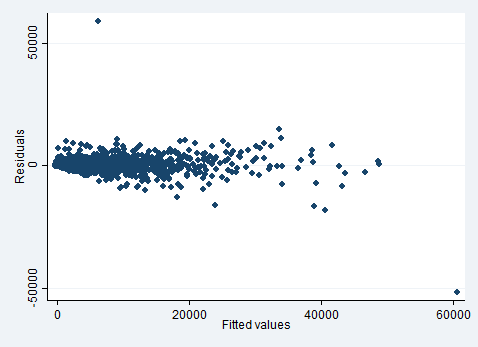
\includegraphics[height=0.3\textheight]{figApp/model-3-ols-residuals}\label{Residual Plots for OLS Models (3)}}
\end{minipage}
\hspace{5cm}
\begin{minipage}{3.3cm}
    \centering
    \subtop[]{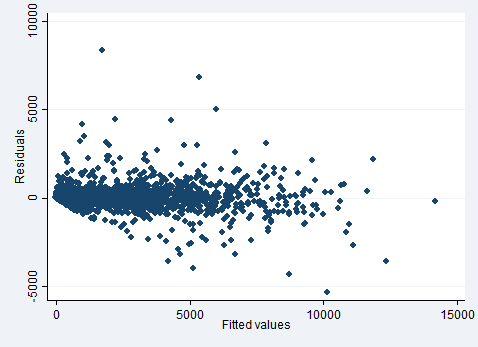
\includegraphics[height=0.3\textheight]{figApp/model-4-ols-residuals}\label{Residual Plots for OLS Models (4)}}
\end{minipage}
\mycaption[Residual Plots for OLS Models (3) and (4).]{(a)~Residual Plots for OLS Models (3). (b)~Residual Plots for OLS Models (4). }
\label{fig:multiRH02}
\end{figure}

\begin{figure}[h]
\begin{minipage}{3.3cm}
    \centering
    \subtop[]{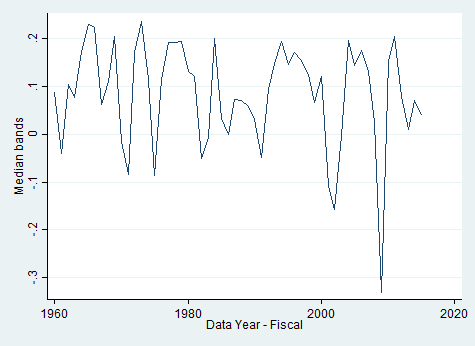
\includegraphics[height=0.3\textheight]{figApp/gr_capx_median_graph}\label{Time series plot of median logged capital expenditures.}}
\end{minipage}
\hspace{5cm}
\begin{minipage}{3.3cm}
    \centering
    \subtop[]{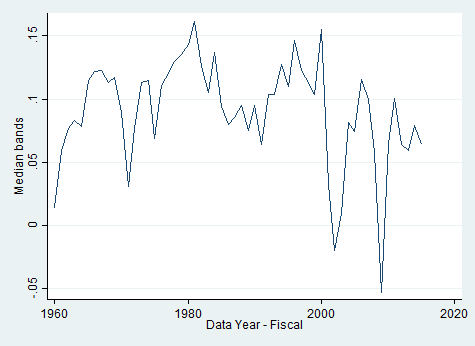
\includegraphics[height=0.3\textheight]{figApp/gr_xrd_median_graph}\label{Time series plot of median logged R and D expenses.}}
\end{minipage}

\begin{minipage}{3.3cm}
    \centering
    \subtop[]{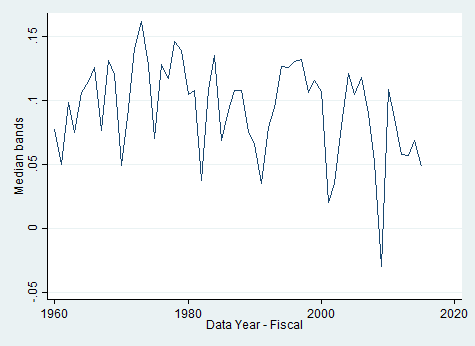
\includegraphics[height=0.3\textheight]{figApp/gr_gp_median_graph}\label{Time series plot of median growth in gross profits.}}
\end{minipage}
\hspace{5cm}
\begin{minipage}{3.3cm}
    \centering
    \subtop[]{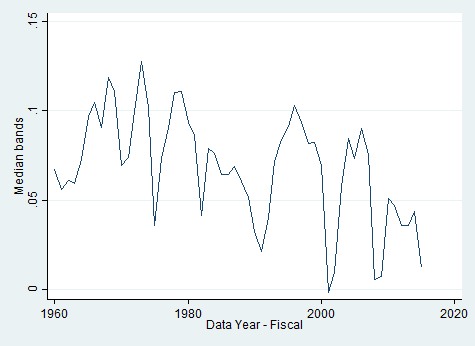
\includegraphics[height=0.3\textheight]{figApp/gr_at_median_graph}\label{Time series plot of median growth in total assets.}}
\end{minipage}

\mycaption[Time Series Plots of First-Differenced Growth Rates in Investment, Assets, and Profit Variables.]{(a)~Time series plot of median first-differenced growth in capital expenditures. (b)~Time series plot of median first-differenced growth in research and development expenses. (c)~Time series plot of median first-differenced growth in gross profits. (d)~Time series plot of median first-differenced growth in total assets. }
\label{fig:multiRH02}
\end{figure}

\begin{table}[h]
\begin{tabular}{ c | c }
	\hline
	\textbf{Corrected Model (3) with Robust Standard Errors} \\
    \textbf{Regressand: Capital Expenditures} \\
    \hline \hline
    Number of Observations & 222,995 \\
	\hline
    $R^{2}$ & 0.2051 \\
    \hline \hline
\end{tabular} \\

\begin{tabular}{ l | c | c | c | c | c }
	\hline
	\textbf{Regressors} & \textbf{Estimators} & \textbf{Std. Errors} & $z$ & $P > |z|$ & 95\% CI \\
    (All in Growth Rates) & $\hat{\beta}$ & $\hat{\sigma}$ & & & \\
    \hline \hline
	Gross Profits & 0.140 & 0.00688  & 20.32 & 0.000 & (0.126, 0.153) \\
	\hline
    Total Assets & 0.900 & 0.0111 & 81.32 & 0.000 & (0.879, 0.922)\\
    \hline
    Capital Expenditures & -0.259 & 0.00304 & -85.12 & 0.000 & (-0.265, -0.253) \\
    (Lagged By 1 Year) & & & & & \\
    \hline \hline
\end{tabular}
\mycaption[GLS Estimations of Corrected Model (3) with Robust Standard Errors]{GLS Estimations of Corrected Model (3) with Robust Standard Errors}
\end{table}

\begin{table}[h]
\begin{tabular}{ c | c }
	\hline
	\textbf{Corrected Model (4) with Robust Standard Errors} \\
    \textbf{Regressand: R\&D Expense} \\
    \hline \hline
    Number of Observations & 82,864 \\
	\hline
    $R^{2}$ & 0.2051 \\
    \hline \hline
\end{tabular} \\

\begin{tabular}{ l | c | c | c | c | c }
	\hline
	\textbf{Regressors} & \textbf{Estimators} & \textbf{Std. Errors} & $z$ & $P > |z|$ & 95\% CI \\
    (All in Growth Rates) & $\hat{\beta}$ & $\hat{\sigma}$ & & & \\
    \hline \hline
	Gross Profits & 0.0871 & 0.00803  & 10.85 & 0.000 & (0.0714, 0.103) \\
	\hline
    Total Assets & 0.306 & 0.00917 & 33.40 & 0.000 & (0.288, 0.324)\\
    \hline
    Capital Expenditures & -0.114 & 0.000851 & -13.36 & 0.000 & (-0.130, -0.0971) \\
    (Lagged By 1 Year) & & & & & \\
    \hline \hline
\end{tabular}
\mycaption[GLS Estimations of Corrected Model (4) with Robust Standard Errors]{GLS Estimations of Corrected Model (4) with Robust Standard Errors}
\end{table}

\